%File: formatting-instruction.tex
\documentclass[letterpaper]{article}
\usepackage{aaai}
\usepackage{times}
\usepackage{helvet}
\usepackage{courier}
\usepackage{graphicx}
\frenchspacing
\setlength{\pdfpagewidth}{8.5in}
\setlength{\pdfpageheight}{11in}
\def\mydoubleq#1{``#1''}
\def\mysingleq#1{`#1'}
\usepackage{amsmath}
\pdfinfo{
/Title ( Error Classification in OCR Historic Newspaper Archive using SVM\textsuperscript{multiclass})
/Author (Megha Gupta, Dr. Haimoti Dutta)}
\setcounter{secnumdepth}{1}  
 \begin{document}
% The file aaai.sty is the style file for AAAI Press 
% proceedings, working notes, and technical reports.
%
\title{Error Classification in OCR Historic Newspaper Archive using multi-class Support Vector Machine}

%\author{Megha Gupta\\Department of Computer Science,\\ IIIT-Delhi, India \\ meghag@iiitd.ac.in 
%\And Dr. Haimonti Dutta\\
%Center for Computational Learning Systems,\\ Columbia University, New York\\ haimonti@iiitd.ac.in}

\author{Megha Gupta and Haimonti Dutta*\\
Department of Computer Science, IIIT-Delhi\\
**Affiliated to The Center for Computational Learning Systems, Columbia University, New York\\
(meghag, haimonti)@iiitd.ac.in
}

\maketitle
\begin{abstract}
\begin{quote}
\noindent Optical Character Recognition (OCR) is a commonly used method of digitizing printed texts so that they can be searched and displayed online, stored compactly and used in text mining applications.\\
The text generated from OCR devices, however, is often garbled due to variations in quality of the input paper, size and style of the font and column layout. This adversely affects retrieval effectiveness; hence the techniques for cleaning the OCR need to be improvised. Often such techniques involve laborious and time consuming manual processing of data.\\
This paper shows the need to devise an algorithm that is scalable for a large dataset. The current state of the art algorithm used for performing multi class classification is not yet scalable. The current algorithm takes a long time to converge in a particular parameter setting.

\end{quote}
\end{abstract}

\section{Introduction}
\label{sec:intro}

The \textit{California Digital Newspaper Collection}\footnote{http://cdnc.ucr.edu/cgi-bin/cdnc} is an initiative of the Center for Bibliographical Studies and Research (CBSR) which is supported in part by the U.S. Institute of Museum and Library Services and National Endowment for the Humanities (NEH) to digitise California newspapers for the National Digital Newspaper Program (NDNP). It contains over 400,000 pages of significant historical California newspapers published from 1846-1922.\\
OCR devices are widely used in electronic conversion of scanned images which are handwritten or printed text into a machine encoded text. The scanning generates  It finds most successful applications in the field of machine Learning, Artificial Intelligence and Pattern recognition. It deals with the problem of recognising optically generated characters be it offline or online. The performance directly depends on the quality of input document. The more constrained the input is the better will be the performance of the system. But when it comes to unconstrained handwriting, the performance is far from satisfactory. The main application areas for \cite{OCR} like Automatic number plate readers, form readers, signature verification.\\
This project deals with printed text in the form of Historical Newspaper Articles in the holdings of \cite{cdnc}. One such newspaper, The Amador Ledger published in the early 1900s by the Amador Publishing Company appealed to the community's interests by covering issues unique to gold mining. Patrons of the \cite{cdnc} continue to be interested in studying about the status of the local mining industry and consequently read the Amador Ledger on a regular basis even to this day and correct \cite{OCR} errors as they come across them.\\
In this paper, we perform error classification using Joachims multi-class Support Vector Machine algorithm called \textit{SVM\textsuperscript{multiclass}}\footnote{http://www.cs.cornell.edu/people/tj/svm\_light/svm\_multiclass.html}. We chose this algorithm as its the state of the art algorithm till now. But the experiments give altogether a different view on this algorithm. This algorithm do not converge quickly on certain parameters which are shown in table ~\ref{table: runtime}

\section{Related Work}
\label{sec:related}
\subsection{OCR correction}
The OCR enables searching of full text data but it is not 100\% accurate. Its accuracy largely depends on paper quality of the original issue, font style, column layouts, its condition at the time of microfilming, choice of scanner \cite{issue}, and the quality of the OCR software. The OCR errors are widely classified as non-word errors and real-word errors. A non-word error takes place when the erroneous word is not a dictionary word whereas in real-word error the erroneous word is correctly spelt and therefore can be found in the dictionary but incorrectly used in context. A related work on the OCR error classification is done by \cite{post-correction}. It gives a more exhaustive classification with respect to OCR errors that helps in classifying real words not contained in any of the dictionary, e.g. names, out-dated or historic spelling variations. Segmentation errors, Hyphenation error, Misrecognition of characters, Punctuation errors, Case sensitivity, Changed word meaning are the classes required for better classification of OCR errors.

%The OCR errors are usually dependent on some major factors like the page quality, text layout, font styles. In \mydoubleq{Issues in automatic error correction}, the experimental analysis has shown that there is another important factor that impacts the performance of the OCR errors which is the choice of scanners used to scan the printed text. The type of scanner used not only affect the quantity of errors but quality as well. Their algorithm for classifying OCR errors is based minimising the cost of basic operations used to transform one string to another, also known as edit distance using dynamic programming approach.\\
%\mydoubleq{Unsupervised Post Correction} paper talks about the post processing of OCR text to minimise the errors. It uses a combination of Anagram Hashing techniques, bigram approach on word level to consider the context and a  similarity key technique called OCR-key.  Anagram Hashing technique uses a hashing function that assigns same number to all those words that have same characters. OCR key observes the shape of characters to know the nature of OCR system and its generated errors.

\subsection{Multi-class SVM}
SVMs are inherently binary classifiers. To solve the multi class problem, construction of several binary classifiers is required and the result from each classifier is combed. The traditional approaches to do multi class classification are:
a) \textit{one-versus-all (OVA classification)} classifies the new instances is done by winner-takes-all strategy where the classifier with highest output function assigns the label. It generates k classifiers for a k class problem.
b)\textit{one-versus-one} uses the majority voting strategy where each classifier assigns the new instance one of the two class, thereby increasing the vote of the assigned class. Finally the class with the majority votes determines the instance classification.
It generates k(k-2)/2 models for a k class problem. This approach is not practical for large-scale classification because of the memory required for storing k(k-1)/2 models.
c)\textit{Directed Acyclic Graph SVM}
d)\textit{error correcting output codes}\\
The other alternative is by using \textit{pairwise classification} \cite{pairwise}, where a two class classifier is build on the two input example. The class of training example might be unknown but the mandatory condition is to know whether the examples belong to the same class or not. The input pair is positive pair when the both belong to the same class, otherwise its called as negative pair. \\
The \cite{crammer} approach was to pose the multi class classification problem into a single optimization problem, rather than decomposing it into multiple binary classification problems.

\section{The Data}
\label{sec:data}

\subsection{Newspaper}
Figure ~\ref{fig:issue} shows a scanned newspaper (\textit{The Amador Ledger}, January 26,1900) from the \cite{cdnc} archive highlighting the article to be corrected by the user. The raw OCR text of the highlighted article is  displayed by clicking on the specific article headline from the list of headlines seen on the left side of the issue in figure ~\ref{fig:issue}. 

%The OCR text generated by running the OCR device on the scanned images of the newspaper was downloaded from the website using Python scripts. The general idea was to decode the names of the log files to retrieve the newspaper name and date. These were further used to formulate URLs needed to download the corresponding OCR text. For instance, \mydoubleq{AL19000105-changes.log} was converted to Amador Ledger, 1900-01-05 which was further translated to \textit{http://chroniclingamerica.loc.gov/lccn/sn93052980/1900-01-05/ed-1/seq-1/ocr.txt}.\\
%Here, seq-1 refers to the first page in the sequence of pages in the newspaper. Therefore to extract issues of Amador Ledger, the only thing varied was date.
%The old and its corresponding new text were stored as key value pairs of a dictionary. Once all the pairs were generated from a log file, the text in the raw corpus matching the keys of the dictionary was replaced with the value corresponding to the matched key.\\
%An analysis was done to figure out the effects of noisy data on text retrieval. The experiments were run on the indexes created on both the datasets using the same query set. The documents retrieved were ranked according to the frequency of the keyword present in the document. Higher the frequency, higher the ranking order. We used Spearman correlation coefficient as the metric to measure the similarity between both our corpora. The average value of Spearman's ranked correlation coefficient calculated by our experiments was 0.625 which denotes that the association between the two corpora is not very strong but the positive value shows that if Raw OCR increases then Corrected OCR will definitely increase.\\

\begin{figure}[ht!]
\centering
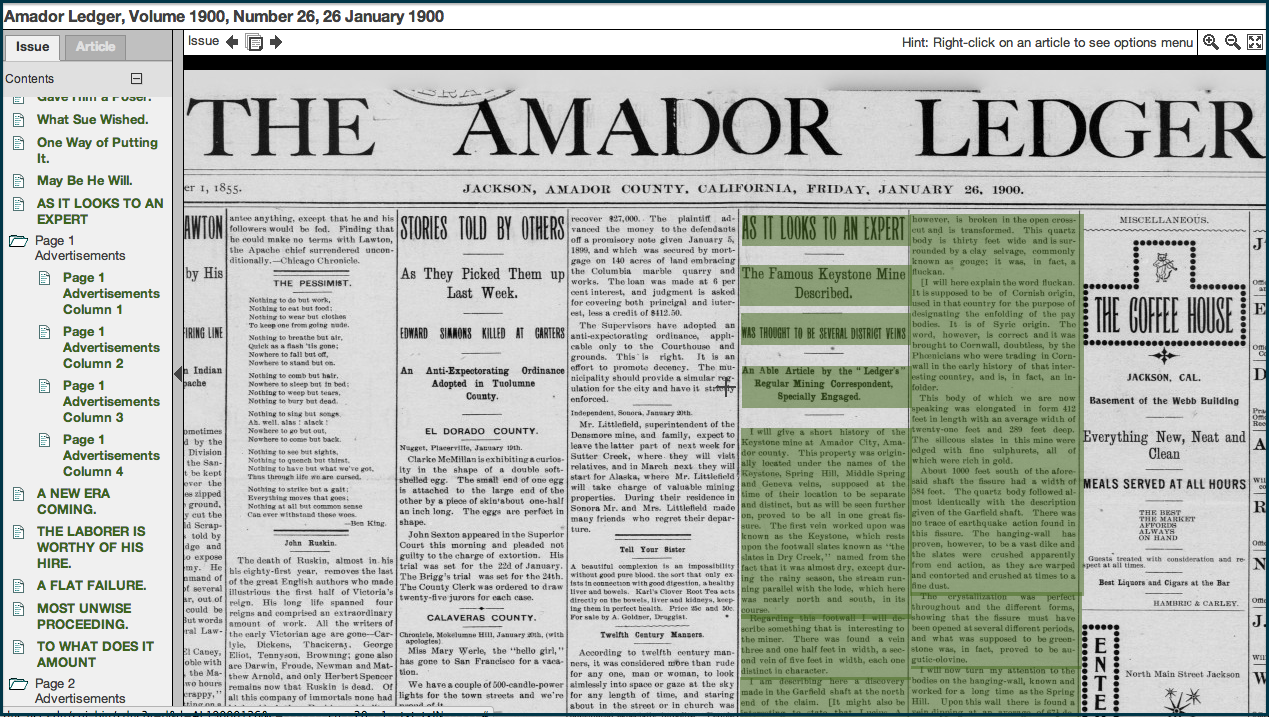
\includegraphics[width=7cm,height=4cm]{./image/issue.png}
\caption{Amador Ledger}
\label{fig:issue}
\end{figure}

The tool used by patrons to correct OCR text is shown in figure ~\ref{fig:correction}. All the corrections performed by the annotators were recorded in the log files.
\begin{figure}[ht!]
\centering
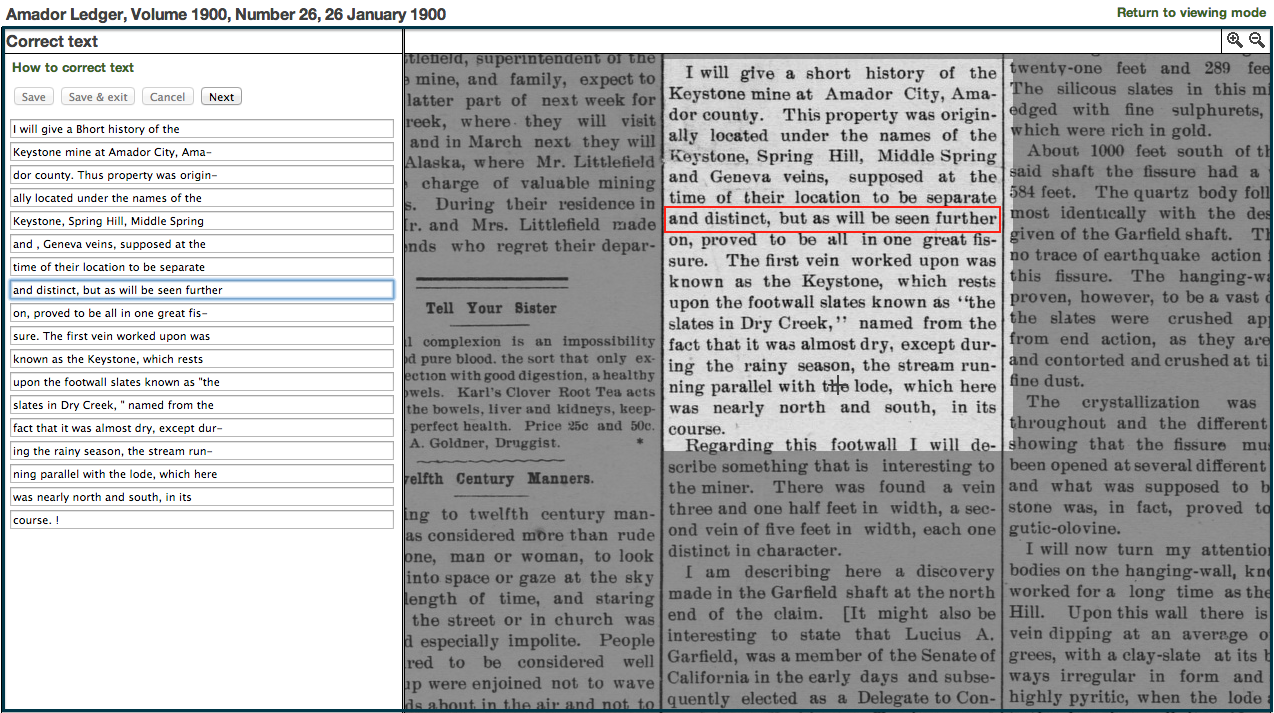
\includegraphics[width=7cm,height=4cm]{./image/correction.png}
\caption{Text correction tool}
\label{fig:correction}
\end{figure}

The text correction statistics consisting of total number of annotators involved in the the data enrichment process are shown in figure ~\ref{fig:annotators}. The total number of lines corrected by 848 users are 1,705,149.
\begin{figure}[ht!]
\centering
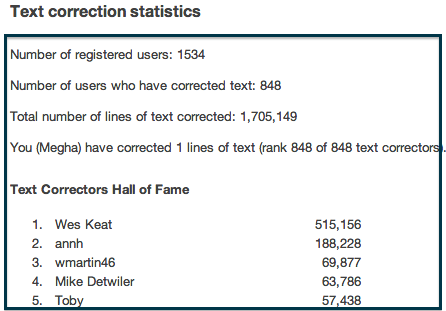
\includegraphics[width=6cm,height=4cm]{./image/annotators.png}
\caption{Text correction statistics}
\label{fig:annotators}
\end{figure}

\subsection{Log-files}
The log files are the files that maintain the history of raw OCR and its corresponding corrected OCR text. These files were generated using a third party software issued by \textit{Veridian}\footnote{http://www.dlconsulting.com/}, a digital library software. Each of the log file was generated at an issue-level, containing xml data about the multiple pages in the issue. The table ~\ref{table:logfile} describes the structure and the format of the log file. The following information is provided about the corrections made by the patrons:\\
a) \textit{Page Id} representing the id of the page in which editing was done.
b) \textit{Block Id} representing the id of the paragraph containing the line corrected by the user.
c) \textit{Line Id} is the id of the particular line edited by the user.
d) \textit{Old text} is the garbled text generated by the OCR device and replaced by the user.
e) \textit{New text} is the corrected text with which the old text was replaced.

\begin{table}[htdp]
\begin{center}
\begin{tabular}{l}
\textless TextCorrectedLine lineID="P2\_TL00800"\textgreater \\
\textless OldTextValue\textgreater \textbf{Spll, Stales}\textless /OldTextValue\textgreater \\
\textless NewTextValue\textgreater \textbf{Union Stables}\textless /NewTextValue\textgreater \\
\textless /TextCorrectedLine\textgreater \\
\textless TextCorrectedLine lineID="P2\_TL00801"\textgreater \\
\textless OldTextValue\textgreater \textbf{**?�** Under Webb Hall *}\textless/OldTextValue\textgreater \\
\textless NewTextValue\textgreater \textbf{Under Webb Hall} \textless/NewTextValue\textgreater \\
\textless /TextCorrectedLine\textgreater \\
\end{tabular}
\end{center}
\caption{A segment of the log file}
\label{table:logfile}
\end{table}

There were in total 235 log files of which we worked on 191. 
% To get an idea of the number of corrections made by a user per log file, a histogram is shown in figure ~\ref{fig:histogram} 

%The names of the log files follow a convention; the first two letters represent the initials of the newspaper followed by the date in the format yyyymmdd. For example \mydoubleq{AL19000105-changes.log} expands to Amador Ledger, 1900-01-05. 

%\begin{figure}[ht!]
%\centering
%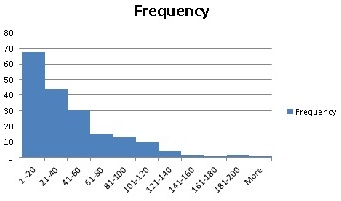
\includegraphics[width=7cm,height=5cm]{./image/histo.jpg}
%\caption{Histogram}
%\label{fig:histogram}
%\end{figure}
\subsection{Preprocessing}
In order to make use of the full text data, we did some preprocessing on the data stored in the log files. We extracted the old text and the corresponding new text from the log file and tokenized them into words. These tokens were separated by whitespaces. There were in total 44,023 tokens of which 21,113 were corrected by the annotators. The errors rectified by the users were categorized as spellcheck error , addition of a new word, capitalization error, typo, punctuation error. The distribution of the these classes in the dataset is shown in figure ~\ref{fig:stats}


\begin{figure}[h]
\centering
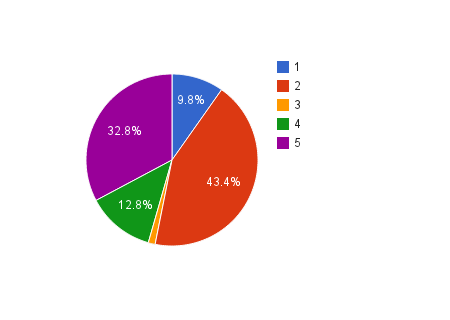
\includegraphics[width=7cm,height=5cm]{./image/error.png}
\caption{Error Classification}
\label{fig:stats}
\end{figure}


\section{Methodology}
\label{sec:methodology}
%Theory about the SVM
We are performing automatic text correction by modelling it through a machine learning algorithm, called multi class Support Vector Machines \cite{algo}. In this formulation, multi class problem is posed as a constrained optimization problem with a quadratic objective function.
The multi class formulation is stated as\\
\begin{equation}
min 1/2 \sum_{i = 1}^{k} w_{i}*w_{i} + C/n \sum_{i = 1}^{n}\xi_{i} 
\end{equation}
\begin{equation*}
s.t. \forall y \leq k : [x_{1} \cdot w_{yi}] \geq [x_{1} \cdot w_{y}] + 100*\Delta(y_{1},y)-\xi_{1}
\end{equation*}
 . . . . . . . . . . .
\begin{equation*}
s.t. \forall y \leq k : [x_{n} \cdot w_{yn}] \geq [x_{n} \cdot w_{y}] + 100*\Delta(y_{n},y)-\xi_{n} 
\end{equation*}
Here C is the regularization parameter that trades off margin error and training error. $\Delta(y_{1},y)$ is the loss function that returns 0 if $y_{n}$ equals y, and 1 otherwise. $\xi_{i}$ are the non negative slack variables which measure the degree of misclassification of the data $x_{i}$. \\
\cite{algo} has to two modules, \textit{svm\_multiclass\_learn} and \textit{svm\_multiclass\_classify}. The learning module learns the model given the parameters and the training data whereas the classification module applies the learned model to the test data to find the error. When the data is not linearly separable, the original finite dimensional space is mapped to a much higher dimensional space in order to make the separation easier in that space. The mappings used by SVM schemes are designed to ensure that the dot products may be computed easily in terms of the variables in the original space, by defining them in terms of a Kernel function selected to suit the problem. The types of kernel function used can be described as follows:\\
a) Linear Kernel (default) : It is the basic kernel function given by the inner product \textless x,y\textgreater plus an optional constant c. K(x,y) = $x^{T}$y + c \\
b) Polynomial Kernel : It is a non-stationary kernel which is well suited for problems where the training data is normalized. \\
K(x,y) = $(\alpha x^{T}y + c)^{d}$ \\
c) Radial Basis Kernel : The (Gaussian) radial basis function kernel on two samples x and y represented as feature vectors in some input space is defined as \\
K(x,y) = exp($-\lvert \lvert x-y\rvert\rvert^{2}$/2$\sigma^{2}$)



%SVM is a state-of-the art algorithm with a strong theoretical foundation based on  Vapnik-Chervonenkis theory \cite{vapnik}.
%SVMs are useful tool when the data is irregularly distributed or have unknown distribution. They provide good out-of-sample generalization if some of the parameters %C and r (in case of Gaussian)% 
%are appropriately chosen. Therefore, they can be robust even when the training sample has some bias. Also they guarantee a unique solution as the optimality problem is convex.



\section{Empirical Evaluation}
\label{sec:evaluation}

\subsection{Preprocessing \& Data Generation}

\subsubsection{Feature Construction} %correct the first line
Originally, there were two features in the dataset, that is old text and new text. Further features were manually crafted looking at the types of errors. In our dataset, we have six binary features consisting of SameLength, EditDist\_0, EditDistAbove1, EditDistBelow3, EditDist\_1andCaseChange, PunctuationDiff.
\begin{enumerate}
\item \mydoubleq{SameLength} is 1 if  both the old word and new word have same length
\item \mydoubleq{EditDist\_0} is 1 if both the words are exactly same
\item \mydoubleq{EditDistAbove1} is 1 if more than one edit operation is required to convert old word to new word
\item \mydoubleq{EditDistBelow3} is 1 if less than three edit operations are required to convert old word to new word
\item \mydoubleq{EditDist\_1andCaseChange} is 1 if the two words have edit distance is exactly 1 and the first character of one string change from upper case to lower case or vice versa.
\item \mydoubleq{PunctuationDiff} is 1 if both the old text and new text differ in any of the following punctuation marks !"\#\$\%\&'()*+,-./:;\textless=\textgreater?@[$\backslash$]\^\_`\{\textbar\}\textasciitilde
\end{enumerate}

\subsubsection{Label Construction}
The error classes were restricted to 6 classes including Spellcheck Error, Addition of a new word, Capitalization Error, Typo, Punctuation Error and No correction
These labels were assigned according to the flow graph as shown in figure
\begin{enumerate}
\item Spellcheck error : When the edit distance is between 1 and 3. For example, mounten and mountain.
\item Addition of a new word : When the edit distance is more than 3. For example, at and attend.
\item Capitalization error : When the edit distance of two strings is exactly 1 and first letter of both the strings changes from upper to lower case or vice versa. For example, largest and Largest.
\item Typo : When the edit distance is exactly one and case change is 0. For example, teh and the
\item Punctuation error : When the two strings differ by special characters contained in the set (!"\#\$\%\&'()*+,-./:;\textless=\textgreater?@[$\backslash$]\^\_`\{\textbar\}\textasciitilde). For example, \mydoubleq{residents} and residents
\item No correction :  When the old and new text are same. For example, plant and plant
\end{enumerate}

The dataset was parsed to a format used by the Joachim's multi class SVM algorithm which is represented as\\
\textless target\textgreater\space\textless feature\textgreater:\textless value\textgreater ......\textless feature\textgreater:\textless value\textgreater\\
The number of rows in the dataset is 44,022. The class distribution in the dataset is shown in table ~\ref{table: classes}
\begin{table}[htdp]
\begin{center}
\begin{tabular}{| c | c |}
\hline
$ Class $ & $ no. of instances $ \\
\hline
1 & 1970 \\
\hline 
2 & 8732 \\
\hline
3 & 261 \\
\hline
4 & 2572 \\
\hline
5 & 6602 \\
\hline
6 & 23885 \\
\hline
Total & 44022 \\
\hline
\end{tabular}
\end{center}
\caption{Class Distribution}
\label{table: classes}
\end{table}



\subsection{Experiment Setup}

Experiments were performed by randomly partitioning the data into 70\% (30,815 instances) and 30\% (13,207 instances) of training and testing data respectively. For each experiment, the regularization parameter (C) and the type of kernel (t) was varied to (0.001,0.01,0.1,1,10,100) and (Linear, Polynomial and Radial basis kernel) respectively. The experiments were performed on two machines, one of which was a linux server and the other was a dual core Mac machine with Intel Core i7 processor, 8GB RAM, 2.9 GHz of processor speed. Each experiment was ran for 5 iterations. The average loss on the test set and CPU runtime were noted to analyse the experiments. Table ~\ref{table: error} describes how the average loss on test set varies for different values of \mysingleq{C} and \mysingleq{t}. Here, $AE_{L}$, $AE_{P}$, $AE_{R}$ describes the average loss error of linear, polynomial and rbf kernels respectively. Table ~\ref{table: runtime}  shows the average runtime (cpu sec) required to learn a model for various values of C and for different kernels. Here, $AT_{L}$, $AT_{P}$, $AT_{R}$ refers to the average run time of linear, polynomial and rbf kernels respectively.
 
\subsection{Results}

\begin{table}[htdp]
\begin{center}
\begin{tabular}{| c | c | c | c |}
\hline
C & $AE_{L}$ & $AE_{P}$ & $AE_{R}$ \\
\hline
.001 & 32.06 $\pm$0.149  & 32.06$\pm$0.149 & 11.96$\pm$0.101 \\
.01 & 32.06$\pm$0.149 & 32.06$\pm$0.149 & 12.04$\pm$0.199 \\
.1 & 32.06$\pm$0.149 & 29.10$\pm$0.133  & 12.04$\pm$0.199  \\
1 &29.10$\pm$0.133  & 28.99$\pm$0.264  & 6.36$\pm$0.142  \\
10 & 29.20$\pm$0.133 & 8.338$\pm$0.107 & 6.36$\pm$0.142 \\
100 & 29.20$\pm$0.133 & 0.58$\pm.034$ & 6.35$\pm0.16$  \\
\hline
\end{tabular}
\end{center}
\caption{Experiment Results : Average loss error (test set)}
\label{table: error}
\end{table}


\begin{table}[htdp]
\begin{center}
\begin{tabular}{| l | c | c | l |}
\hline
C & $ AT_{L} $ & $AT_{P}$ & $AT_{R}$ \\
\hline
.001 & 0.218 & 5192 & 4596 \\
.01 & 0.202 & 5166 & 4460 \\
.1 & 0.208 & 72225 & 4377 \\
1 & 0.678 & 81251 & 16468 \\
10 & 0.672 & 260316 & 55308 \\
100 & 0.998 & 106753  & 48734  \\
\hline
\end{tabular}
\end{center}
\caption{Experiment Results : Training time (cpu sec)}
\label{table: runtime}
\end{table}

\subsection{Discussion}
As can be seen in table ~\ref{table: error} , the error is minimum when the C = 100 and when the kernel type is polynomial. But the time taken as shown in table ~\ref{table: runtime} to train the model for these parameters, when C is 100 is 106753 cpu sec.
\subsection{Known Defects}
The \cite{algo} algorithm converges quickly for linear type kernel but the its performance on test set is poor. For non linear kernels, this algorithm does not scale well for large scale datasets but gives better performance than linear kernels.

\section{Conclusion \& Future Work}
The California Digital Newspaper Collection has an archive of 400,000 pages of historical California newspapers published between 1846 to 1922. This archive which has been subjected to OCR and is currently stored in an online database making them accessible to patrons. The OCR scanning process generates lot of garbled text which needs to be corrected to make the online newspaper repository more accessible to general public. An automatic OCR error correction technique is implemented using machine learning technique, multi class Support Vector Machine used to build a model for predicting errors in the dataset generated. State-of -the-art algorithm \cite{algo} was used to for our experiments to predict the errors. The labels generated using the approach mentioned in section ~\ref{sec:evaluation} served as the ground-truth against which labels generated by the algorithm were compared. Our results indicate that even the state-of-the-art algorithm is not scalable for large scale learning as it takes 106753 cpu sec to learn a model on data with 30,185 instances.
Our Future work involves careful analysis of the current algorithm to scale the non-linear kernels for large scale learning.




% use section* for acknowledgement
\section*{Acknowledgment}
This work is supported by funding from the National Endowment for Humanities. I would also like to express my gratitude to my Advisor, Dr. Haimonti Dutta for her support, patience and encouragement throughout the research.\\

\nocite{carlson,wikiedits,massive,Gao,Huang,hoi2006large,menon2009large,notes,Thorsten,DBLP:journals/csur/Kukich92,Reynaert2008a,Niklas2010,Tong96astatistical,post-correction}

\begin{quote}
\begin{small}
\bibliographystyle{aaai}
\bibliography{flairsPaper}
\end{small}
\end{quote}

%\nocite{joachims,pairwise,crammer,issue,thesis,cdnc,digital,OCR,eval,noisy,svm,vapnik,multiclass}



\end{document}
